\documentclass[addpoints,spanish, 12pt,a4paper]{exam}
%\documentclass[answers, spanish, 12pt,a4paper]{exam}
%  \printanswers
\pointpoints{punto}{puntos}
\hpword{Puntos:}
\vpword{Puntos:}
\htword{Total}
\vtword{Total}
\hsword{Resultado:}
\hqword{Ejercicio:}
\vqword{Ejercicio:}

\usepackage[utf8]{inputenc}
\usepackage[spanish]{babel}
\usepackage{eurosym}
%\usepackage[spanish,es-lcroman, es-tabla, es-noshorthands]{babel}
\usepackage{pgf,tikz}


\usepackage[margin=1in]{geometry}
\usepackage{amsmath,amssymb}
\usepackage{multicol}
\usepackage{yhmath}

\pointsinrightmargin % Para poner las puntuaciones a la derecha. Se puede cambiar. Si se comenta, sale a la izquierda.
\extrawidth{-2.4cm} %Un poquito más de margen por si ponemos textos largos.
\marginpointname{ \emph{\points}}

\usepackage{graphicx}

\graphicspath{{../img/}} 

\newcommand{\class}{4º Académicas}
\newcommand{\examdate}{\today}
\newcommand{\examnum}{Examen final 2ª evaluación}
\newcommand{\tipo}{A}


\newcommand{\timelimit}{50 minutos}

\renewcommand{\solutiontitle}{\noindent\textbf{Solución:}\enspace}


\pagestyle{head}
\firstpageheader{
\includegraphics[width=0.2\columnwidth]{header_left}}{\textbf{Departamento de Matemáticas\linebreak \class}\linebreak \examnum}{
\includegraphics[width=0.1\columnwidth]{header_right}}
\runningheader{\class}{\examnum}{Página \thepage\ of \numpages}
\runningheadrule

\DeclareUnicodeCharacter{2212}{-}
\begin{document}

\noindent
\begin{tabular*}{\textwidth}{l @{\extracolsep{\fill}} r @{\extracolsep{6pt}} }
\textbf{Nombre:} \makebox[3.5in]{\hrulefill} & \textbf{Fecha:}\makebox[1in]{\hrulefill} \\
 & \\
\textbf{Tiempo: \timelimit} & Tipo: \tipo 
\end{tabular*}
\rule[2ex]{\textwidth}{2pt}
Esta prueba tiene \numquestions\ ejercicios. La puntuación máxima es de \numpoints. 
La nota final de la prueba será la parte proporcional de la puntuación obtenida sobre la puntuación máxima. 

\begin{center}


\addpoints
 %\gradetable[h][questions]
	\pointtable[h][questions]
\end{center}

\noindent
\rule[2ex]{\textwidth}{2pt}

\begin{questions}


% \question[1] 
% \begin{solution} \end{solution}
% \addpoints


\question Resuelve la siguiente inecuación racional:\begin{parts} 
\part[2] $\dfrac{x^{2} - 4}{x^{2} - 9} \geq  0$\begin{solution} $\left(-\infty, -3\right) \cup \left[-2, 2\right] \cup \left(3, \infty\right)$\end{solution} 
% \part[2] $\dfrac{x^{2} -4x +4}{x^{2} - 1} \geq  0$\begin{solution} $\left(-\infty, -1\right) \cup \left(1, \infty\right)$\end{solution} 
% \part[2] $\dfrac{x^{2} - 4}{x^{2} - 9} \leq  0$\begin{solution} $\left(-3, -2\right] \cup \left[2, 3\right)$\end{solution} 
% \part[2] $\dfrac{x^{2} -2x +1}{x^{2} - 9} \leq  0$\begin{solution} $\left(-3, 3\right)$\end{solution} 
\end{parts} 


\question Resuelve la siguiente inecuación con valor absoluto:\begin{parts} 
\part[2] $| {2x - 4} | \leq  8$\begin{solution} $\left[-2, 6\right]$\end{solution} 
% \part[1] $| {2x + 3} | < 5$\begin{solution} $\left(-4, 1\right)$\end{solution} 
% \part[1] $| {3 - 2x} | \leq 7$\begin{solution} $\left[-2, 5\right]$\end{solution} 
\end{parts} 


% \question Resuelve el siguiente sistema de inecuaciones con dos incógnitas (puedes usar el plano cartesiano que se adjunta):

% \begin{parts} 
% \part[2] $\left\{\begin{matrix}4x+2y \geq 8 \\ -x+2y < 4\end{matrix}\right.$\begin{solution} \\ \scalebox{.99}{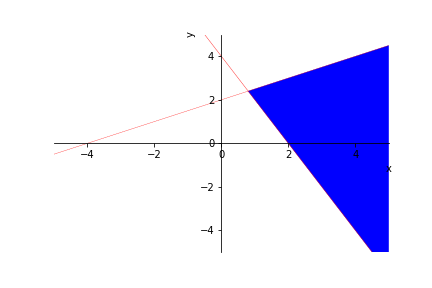
\includegraphics[width=1\columnwidth]{sistema_ine_ex0.png}}\end{solution}

% \part[2] $\left\{\begin{matrix}2x+y \leq 4 \\ 2x-y > 2 \\ y>-2 \\ x>0\end{matrix}\right.$\begin{solution} \\ \scalebox{.99}{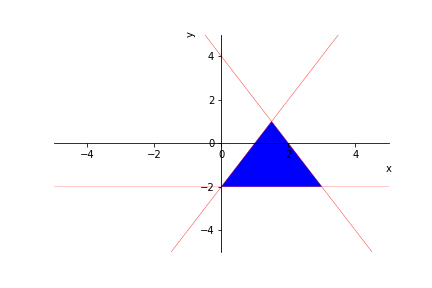
\includegraphics[width=1\columnwidth]{sistema_ine_ex1.png}}\end{solution} 
% \end{parts} 


\question Calcular el dominio de las siguientes funciones:
\begin{parts} 
\part[1] $f(x)=\dfrac{2x+1}{x^{2} - 4 x + 3}$\begin{solution} $\left(-\infty, 1\right) \cup \left(1, 3\right) \cup \left(3, \infty\right)$\end{solution} 
% \part[1] $f(x)=\sqrt{x^2+3x+2}$\begin{solution} $\left(-\infty, -2\right] \cup \left[-1, \infty\right)$\end{solution} 
% \part[1] $f(x)=\dfrac{2x-1}{x^{2} + 4 x + 3}$\begin{solution} $\left(-\infty, -3\right) \cup \left(-3, -1\right) \cup \left(-1, \infty\right)$\end{solution} 
% \part[1] $f(x)=\sqrt{x^{2} - 3 x + 2}$\begin{solution} $\left(-\infty, 1\right] \cup \left[2, \infty\right)$\end{solution} 
\part[1] $f(x)=\dfrac{1}{2-\sqrt{x}}$\begin{solution} $\left[0, 4\right) \cup \left(4, \infty\right)$\end{solution} 
\end{parts} 


% \question Dada la función: $$y=\begin{cases} 3 - 2 x & \text{si}\: x < -1 \\3 & \text{si}\: -1\leq x \leq 3 \\x + 3 & \text{si}\: x>3 \end{cases}$$
% \begin{parts}
% \part[2] Representa la función (puedes usar el plano cartesiano que se adjunta)
% \begin{solution} \scalebox{.6}{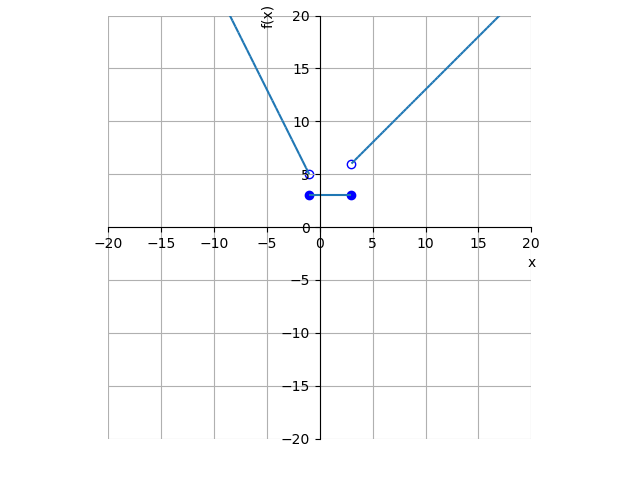
\includegraphics[width=1\columnwidth]{ex_funcion_a_trozos_5}}\end{solution}\part[1] Indica: \begin{itemize}
%     \item Dominio y Recorrido
%     \item Intervalos de crecimiento y decrecimiento
%     \item Máximos y mínimos relativos
%     \item Discontinuidades
% \end{itemize}
% \end{parts}

% \question Dada la función: $$y=\begin{cases} 2 x + 3 & \text{si}\: x < -2 \\3 & \text{si}\: -2\leq x \leq 2 \\3 - x & \text{si}\: x > 2 \end{cases}$$
% \begin{parts}
% \part[2] Representa la función (puedes usar el plano cartesiano que se adjunta)
% \begin{solution} \scalebox{.6}{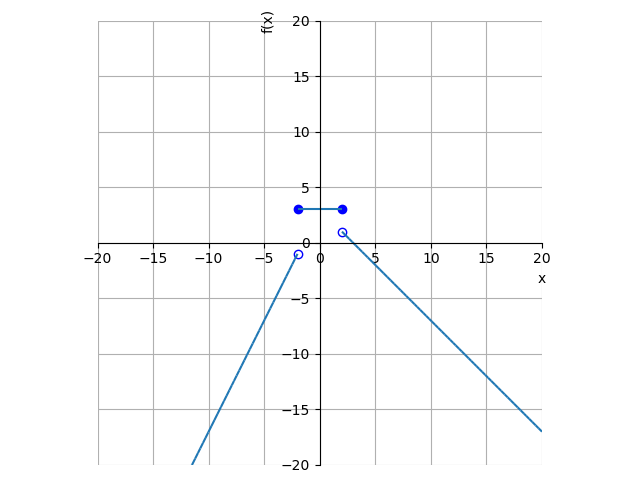
\includegraphics[width=1\columnwidth]{ex_funcion_a_trozos_4}}\end{solution}\part[1] Indica: \begin{itemize}
%     \item Dominio y Recorrido
%     \item Intervalos de crecimiento y decrecimiento
%     \item Máximos y mínimos relativos
%     \item Discontinuidades
% \end{itemize}
% \end{parts}


% \question Dada la función: $$y=\begin{cases} 3 - 2 x & \text{si}\: x < 1 \\- x^{2} + 6 x - 8 & \text{si}\: x \geq 1 \end{cases}$$
% \begin{parts}
% \part[2] Representa la función (puedes usar el plano cartesiano que se adjunta)
% \begin{solution} \scalebox{.6}{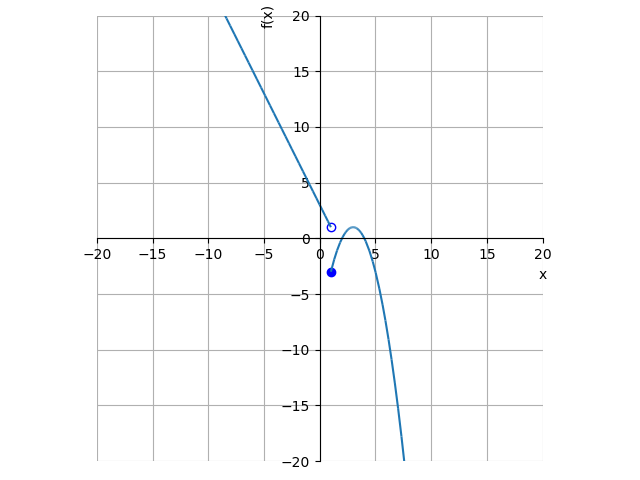
\includegraphics[width=1\columnwidth]{ex_funcion_a_trozos_3}}\end{solution}\part[1] Indica: \begin{itemize}
%     \item Dominio y Recorrido
%     \item Intervalos de crecimiento y decrecimiento
%     \item Máximos y mínimos relativos
%     \item Discontinuidades
% \end{itemize}
% \end{parts}

\question Dada la función: $$y=\begin{cases} 2 x - 3 & \text{si}\: x < -1 \\- x^{2} + 2 x & \text{si}\: x\geq -1 \end{cases}$$
\begin{parts}
\part[2] Representa la función (puedes usar el plano cartesiano que se adjunta)
\begin{solution} \scalebox{.6}{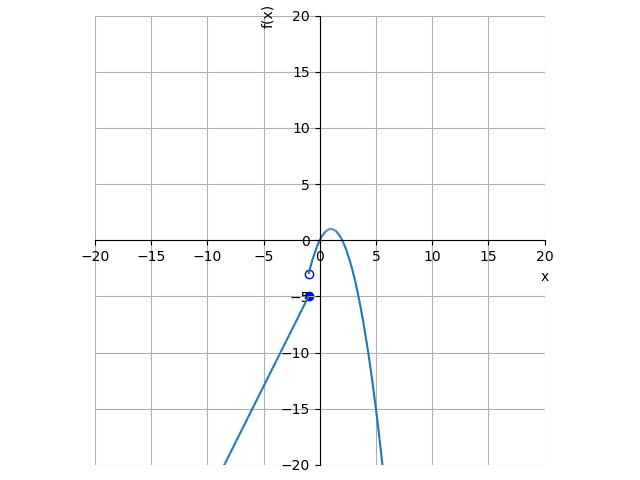
\includegraphics[width=1\columnwidth]{ex_funcion_a_trozos_2}}\end{solution}\part[1] Indica: \begin{itemize}
    \item Dominio y Recorrido
    \item Intervalos de crecimiento y decrecimiento
    \item Máximos y mínimos relativos
    \item Discontinuidades
\end{itemize}
\end{parts}

% \question Dada la función: $$y=\begin{cases} 2 x + 2 & \text{si}\: x \leq -1 \\x^{2} - 2 x &  \text{si} \: x > -1 \end{cases}$$
% \begin{parts}
% \part[2] Representa la función (puedes usar el plano cartesiano que se adjunta)
% \begin{solution} \scalebox{.6}{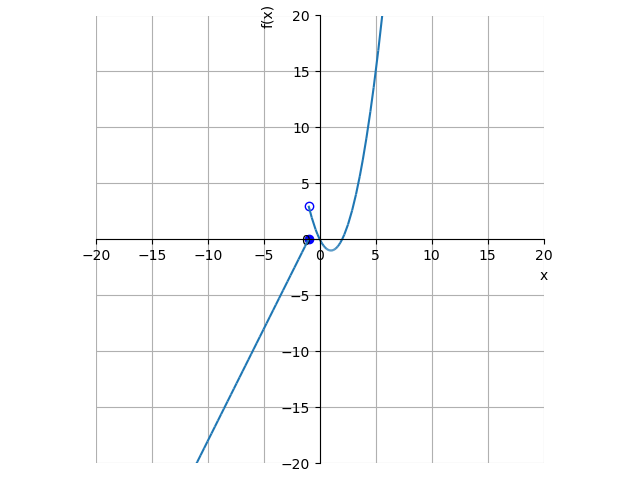
\includegraphics[width=1\columnwidth]{ex_funcion_a_trozos_0}}\end{solution}
% \part[1] Indica: \begin{itemize}
%     \item Dominio y Recorrido
%     \item Intervalos de crecimiento y decrecimiento
%     \item Máximos y mínimos relativos
%     \item Discontinuidades
% \end{itemize}
% \end{parts}

% \question Dada la función: $$y=\begin{cases} 3 - 2 x & \text{si}\: x < 1 \\x^{2} - 6 x + 8 & \text{si}\: x\geq 1 \end{cases}$$
% \begin{parts}
% \part[2] Representa la función (puedes usar el plano cartesiano que se adjunta)
% \begin{solution} \scalebox{.6}{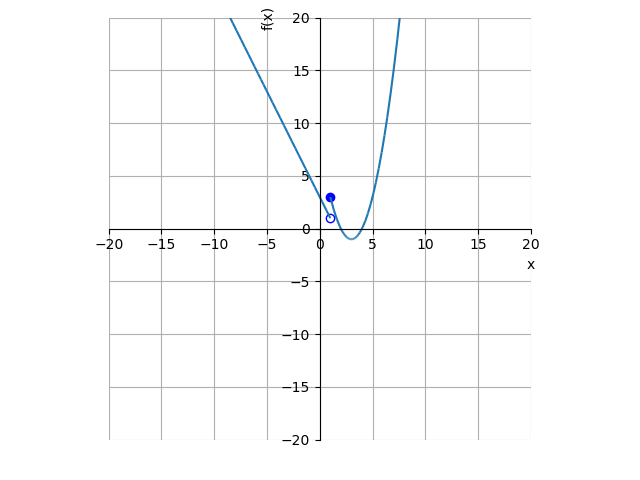
\includegraphics[width=1\columnwidth]{ex_funcion_a_trozos_1}}\end{solution}
% \part[1] Indica: \begin{itemize}
%     \item Dominio y Recorrido
%     \item Intervalos de crecimiento y decrecimiento
%     \item Máximos y mínimos relativos
%     \item Discontinuidades
% \end{itemize}
% \end{parts}


\question[1] Responde a las siguientes cuestiones:
\begin{parts}
\part Indica la ecuación o la expresión analítica correspondiente a una recta que pasa por el punto de coordenadas $\left(0,1\right)$ y cuya pendiente vale 3
\begin{solution}
$y=3x+1$
\end{solution}
\part Razona, sin representar ni calcular puntos de la gráfica, el número de puntos de corte de la función $y=(x-1)^2+1$ con el eje $OX$ 
\begin{solution}
Ninguno, porque $y\geq 1 \ \forall x$
\end{solution}
\end{parts}

\newpage 
% [line cap=round,line join=round,>=triangle 45,x=1cm,y=1cm, scale=0.78]

\begin{tikzpicture}[x=1cm,y=1cm,scale=0.5]
\draw [color=lightgray,dash pattern=on 1pt off 1pt, xstep=1cm,ystep=1cm] (-10.1,-10.1) grid (10.1,10.1);
\draw[color=black] (-10.1,0) -- (10.1,0);
\foreach \x in {-10,-9,-8,-7,-6,-5,-4,-3,-2,-1,1,2,3,4,5,6,7,8,9,10}
\draw[shift={(\x,0)},color=black] (0pt,1pt) -- (0pt,-1pt) node[below] {\footnotesize $\x$};
\draw[color=black] (0,-10.43158220601634095) -- (0,10.1);
\foreach \y in {-10,-9,-8,-7,-6,-5,-4,-3,-2,-1,1,2,3,4,5,6,7,8,9,10}
\draw[shift={(0,\y)},color=black] (2pt,0pt) -- (-2pt,0pt) node[left] {\footnotesize $\y$};
\end{tikzpicture}

\begin{tikzpicture}[x=1cm,y=1cm,scale=0.5]
\draw [color=lightgray,dash pattern=on 1pt off 1pt, xstep=1cm,ystep=1cm] (-10.1,-10.1) grid (10.1,10.1);
\draw[color=black] (-10.1,0) -- (10.1,0);
\foreach \x in {-10,-9,-8,-7,-6,-5,-4,-3,-2,-1,1,2,3,4,5,6,7,8,9,10}
\draw[shift={(\x,0)},color=black] (0pt,1pt) -- (0pt,-1pt) node[below] {\footnotesize $\x$};
\draw[color=black] (0,-10.43158220601634095) -- (0,10.1);
\foreach \y in {-10,-9,-8,-7,-6,-5,-4,-3,-2,-1,1,2,3,4,5,6,7,8,9,10}
\draw[shift={(0,\y)},color=black] (2pt,0pt) -- (-2pt,0pt) node[left] {\footnotesize $\y$};
\end{tikzpicture}


\addpoints

\end{questions}

\end{document}
\grid
